\section{Grappa}
Existing shared memory applications typically do fine-grained operations on data, assuming it is all cheap to access.
Naively translating these applications to PGAS languages often results in poor performance because many operations must then be done via fine-grained remote communication.
Much research has been done to improve performance of PGAS implementations by coming up with better ways to partition data and schedule computation, and do communication in bulk to best utilize network resources.
For workloads with regular access patterns, for instance dense linear algebra or structured grids, there are proven techniques that can automatically optimize communication effectively. \TODO{cite or remove prev. statement}

Irregular applications, on the other hand, are characterized by being highly dependent on the shape of the data, making it difficult to statically partition, causing load imbalance, and requiring a majority of fine-grained random accesses. The goal of the Grappa runtime is to provide a PGAS implementation that has been designed from the ground up to handle such applications.

\begin{figure}[ht]
  \centering
  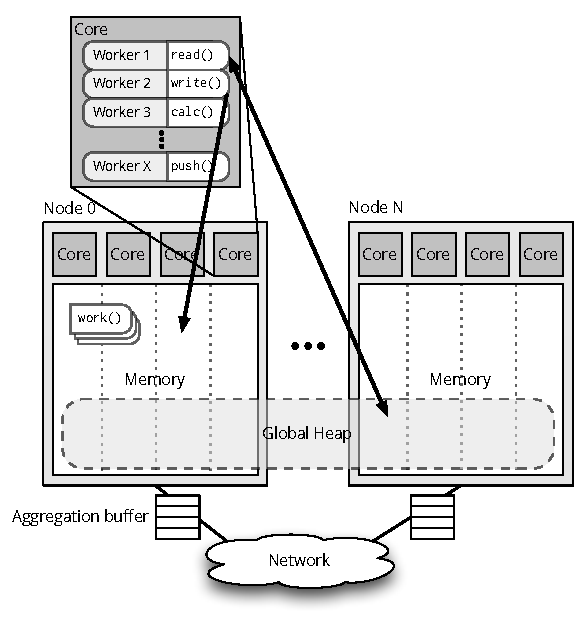
\includegraphics[width=0.5\textwidth]{figs/grappa_system.pdf}
  \caption{\emph{Grappa System Overview:}
    Thousands of workers are multiplexed onto each core, context switching to tolerate the additional latency of aggregating remote operations. Each core has exclusive access to a slice of the global heap which is partitioned across all nodes, as well as core-private data and worker stacks. Tasks can be spawned and executed anywhere, but are bound to a worker in order to be executed.
  }
  \label{fig:system}
\end{figure}

\subsection{Tasks}
\TODO{describe how tasks work}

\subsection{Global Memory}
\TODO{explain how memory is partitioned}

\subsection{Communication}
\TODO{remote delegate operations, aggregation}
